\section{Aritmetica ordinale e forma normale di Cantor}
In questa sezione studieremo nel dettaglio le proprietà delle operazioni aritmetiche fra gli ordinali. Il risultato principale sarà che ogni ordinale $\alpha$ si scrive, in modo unico, nella forma:
\[ \alpha = \omega^{\beta_1}\cdot k_1 + \omega^{\beta_2}\cdot k_2 + \ldots + \omega^{\beta_n}\cdot k_n
	\]
con $n \in \omega$, $k_1,k_2,\ldots,k_n \in \omega\setminus\{0\}$ e $\beta_1 > \beta_2 > \ldots > \beta_n$ (ordinali). Con queste forme normali di Cantor è possibile calcolare le operazioni aritmetiche in modo esplicito.

\begin{note}
	Per procederemo con ordine, assumeremo la definizione ricorsiva delle operazioni ordinali e procederemo unicamente da quella.
\end{note}

\begin{proposition}[Monotonia delle operazioni fra ordinali]
	Le funzioni $(\alpha,\beta)\mapsto \alpha + \beta$, $(\alpha,\beta) \mapsto \alpha \cdot \beta$ e $(\alpha,\beta) \mapsto \alpha^\beta$ sono \textcolor{red}{strettamente crescenti nel secondo argomento} - per $\alpha \cdot \beta$ assumendo $\alpha \ne 0$,
	per $\alpha^\beta$ assumendo $1<\alpha$ - e \textcolor{red}{mai decrescenti [o crescenti debolmente] nel primo argomento}.
\end{proposition}

Per dimostrare la proposizione ci serviranno queste note.

\begin{note}[Condizione sufficiente per la disuguaglianza tra gli estremi superiori]
	Dati due insiemi di ordinali $X,Y$ non vuoti vale che:\footnote{Moralmente: se posso dominare ogni elemento di $X$ con un elemento di $Y$, allora vale la disuguaglianza tra gli estremi superiori.}
	\[ \forall \alpha \in X \; \exists \beta \in Y \; \alpha \leq \beta \rightarrow \sup X \leq \sup Y
		\]
\end{note}

\begin{proof}
	Basta osservare che ogni maggiorante di $Y$ è un maggiorante di $X$, e quindi in particolare si ottiene, dalla definizione di sup di $X$ che $\sup X \leq \sup Y$.\\
	Preso $\alpha \in X$, per ipotesi, esiste $\beta \in Y$ con $\alpha \leq \beta$, e, dato $\gamma$ maggiorante di $Y$, si ha $\alpha \leq \beta \leq \gamma \to \alpha \leq \gamma$,
	per l'arbitrarietà di $\alpha$ abbiamo quindi che $\gamma$ è un maggiorante di $X$, pertanto varrà in particolare che $\sup Y$ è un maggiorante di $X$ e si conclude.
\end{proof}

\begin{note}[Il successore è strettamente crescente]
	La funzione classe $\alpha \mapsto s(\alpha)$ è una mappa strettamente crescente.
\end{note}

\begin{proof}
	$\alpha < \beta \leftrightarrow s(\alpha) \leq \beta \leftrightarrow s(\alpha) < s(\beta)$, dove entrambe le equivalenza corrispondono alle osservazioni sul successore di uno dei due termini di una disuguaglianza.
\end{proof}

Possiamo quindi dimostrare la proposizione.

\begin{proof}
	Vediamo le due richieste nel caso della somma separatamente.\\
	\textcolor{purple}{$\beta \mapsto \alpha + \beta$ è strettamente crescente}\\
	Dobbiamo dire che dati $\beta < \gamma$, vale che $\alpha + \beta < \alpha + \gamma$. Procediamo per \hyperref[induz_transf2]{induzione transfinita v.2} $\gamma$ (cioè quello a più a destra della somma, così da poter usare bene la definizione dell'operazione nel caso limite).
	\begin{itemize}
		\item[$\boxed{\text{caso $\gamma = 0$}}$] Vera a vuoto, poiché $\beta < 0 \leftrightarrow \beta \in \emptyset$.
		\item[$\boxed{\text{caso $\gamma = s(\delta)$}}$] Per ipotesi induttiva abbiamo che $\beta < \delta \rightarrow \beta + \alpha < \beta + \delta$. Preso $\beta < s(\delta)$, questo è equivalente a  $\beta \leq \delta$, da cui, unendo entrambi i casi assieme, si ha:
		\[ \alpha + \beta \leq \alpha + \delta \;\textcolor{red}{<}\; s(\alpha + \delta) \overset{\text{def. ric.}}{=} \alpha + s(\delta) = \alpha + \gamma
			\]
		dove la prima disuguaglianza si ha perché o $\beta = \delta$ o $\beta < \delta$, e quindi in un caso vale l'ipotesi induttiva, nell'altro c'è uguaglianza; la disuguaglianza stretta deriva invece dal fatto visto che il successore è strettamente crescente.
		\item[$\boxed{\text{caso $\gamma = \lambda$ limite}}$] Dato $\beta < \lambda$, abbiamo $s(\beta) < \lambda$ (se così non fosse $\lambda$ sarebbe successore), dunque, possiamo applicare l'ipotesi induttiva a $\beta$ ed a $s(\beta)$, ottenendo:
		\[ \alpha + \beta < s(\alpha + \beta) =  \alpha + s(\beta) \leq \sup\{\alpha + \delta | \delta < \lambda\} = \alpha + \lambda
			\]
		dove per la seconda disuguaglianza è semplicemente la definizione di sup sull'insieme di tutte le possibili somme con secondo termine $<\lambda$, mentre l'ultima uguaglianza è la continuità della somma.
		\end{itemize}
	\textcolor{purple}{$\alpha \mapsto \alpha + \beta$ è non decrescente}\\
	Dobbiamo dire che $\alpha < \gamma$, allora $\alpha + \beta \leq \gamma + \beta$. Procediamo questa volta per \hyperref[induz_transf2]{induzione transfinita v.2} su $\beta$ (che è il termine più a destra della somma).
	\begin{itemize}
		\item[$\boxed{\text{caso $\beta = 0$}}$] Banale per la definizione ricorsiva della somma.
		\item[$\boxed{\text{caso $\beta = s(\delta)$}}$] Per ipotesi induttiva, vale che $\alpha < \gamma \rightarrow \alpha + \delta \leq \gamma + \delta$ e vogliamo dimostrare che $\alpha < \gamma \to \alpha + s(\delta) \leq \gamma + s(\delta)$.
		Usando l'osservazione sulla monotonia del successore fatta prima, e la definizione della somma nel caso successore, si ha:
		\[ \alpha + s(\delta) = s(\alpha + \delta) \;\overset{\text{Hp. indutt. + monoton.}}{\leq}\; s(\gamma + \delta) = \gamma + s(\delta)
			\]
		\item[$\boxed{\text{caso $\beta = \lambda$ limite}}$] Per ipotesi induttiva, se $\delta < \lambda$, allora $\alpha < \gamma \rightarrow \alpha + \delta \leq \gamma + \delta$, dobbiamo verificare che quest'ultima implicazione vale con $\lambda$ stesso al posto di $\delta$
		\[ \alpha + \lambda \overset{(\star)}{=} \sup \{\alpha + \delta | \delta < \lambda\} \leq \sup\{\gamma + \delta | \delta < \lambda\} \overset{(\star)}{=} \gamma + \lambda
			\]
		dove $(\star)$ vale per la continuità della somma ordinale e la disuguaglianza larga al centro è il lemma della disuguaglianza dei sup, la cui ipotesi è soddisfatta dall'ipotesi induttiva.
	\end{itemize}
	Le dimostrazioni per il prodotto e l'esponenziale ripetono pedissequamente lo schema delle precedenti, restano quindi per \underline{esercizio}. Unica osservazione:
	nel passo induttivo del prodotto si deve usare il risultato per la somma, e nel passo induttivo dell'esponenziale si deve usare il prodotto.
\end{proof}

\begin{exercise}
	Le ipotesi che $\alpha \ne 0$ per il prodotto e $1 < \alpha$ per l'esponenziale dove sono usate?
\end{exercise}

\begin{soln}
	Le ipotesi vengono usate nei casi successori rispettivamente del prodotto e della somma nel caso della monotonia stretta nella seconda componente (nel caso della monotonia debole sulla prima non ci sono particolari problemi).
\end{soln}

\begin{remark}[Controesempio alla stretta crescenza della prima componente]
	Basta considerare $0 + \omega$ e $1 + \omega$, infatti, $\omega$ è ordinale limite, dunque:
	\begin{align*}
		& 0 + \omega = \sup \{0 + n | n < \omega\} = \sup \{n | n < \omega\} = \bigcup \{n | n < \omega\} = \omega \\
		& 1 + \omega = \sup \{1 + n | n < \omega\} = \sup \{s(n) | n < \omega\} = \bigcup \{s(n) | n < \omega\} = \omega
	\end{align*}
	quindi la somma con $\omega$ dà lo stesso risultato, ma $0 < 1$, dunque la somma non è strettamente crescente nella prima componente.\footnote{Un controesempio per il prodotto può essere visto ad esempio con $1 \cdot \omega = 2 \cdot \omega = \omega$, e per l'esponenziale,
	come vedremo nella sezione dedicata alle regole di calcolo in forma normale, lo si può fare con $1^\omega = 2^\omega = \omega^\omega$.}
\end{remark}

\begin{proposition}[Proprietà delle operazioni fra ordinali]
	Dati $\alpha,\beta,\gamma \in \Ord$ valgono le seguenti proprietà:
	\[\begin{split}
		\text{\textcolor{red}{associatività:}} &\quad (\alpha + \beta) + \gamma = \alpha + (\beta + \gamma) \quad (\alpha \cdot \beta) \cdot \gamma = \alpha \cdot (\beta \cdot \gamma)\\
		\text{\textcolor{red}{distributività a sinistra:}} &\quad  \alpha \cdot (\beta + \gamma) = \alpha \cdot \beta + \alpha \cdot \gamma \\
		\text{\textcolor{red}{proprietà delle potenze:}} &\quad {\alpha}^{\beta + \gamma} = \alpha^{\beta} \cdot \alpha^{\gamma} \qquad ({\alpha}^{\beta})^{\gamma} = {\alpha}^{\beta \cdot \gamma}
	\end{split}\]
\end{proposition}

\begin{note}
	Abbiamo già asserito la proposizione corrispondente per i buoni ordinamenti (notare gli uguali al posto dei simboli di isomorfismo in questo caso), ma lasciando la dimostrazione per esercizio.
	Lasceremo comunque parte della dimostrazione per esercizio, ma non invano: è un esercizio più facile.
\end{note}

\begin{remark}[$\sup X \not \in X \implies \sup X$ ordinale limite]
	Dato $X$ un insieme di ordinali, sappiamo che è sempre ben definito $\sup X \in \Ord$, se vale che $\sup X \not \in X$, allora  si ha che $\sup X$ è limite.\footnote{Notare che la freccia opposta
	non è in generale vera, ad esempio prendendo $X = \{\omega\}$, si ha che $\sup X = \omega \in X$.}
\end{remark}

\begin{proof}
	Se per assurdo $\sup X = \alpha + 1$, siccome $\sup X$ non è elemento di $X$ ed è un suo maggiorante, si ha $\forall \beta \in X \; \beta < \alpha + 1$,
	cioè $\forall \beta \in X \; \beta \leq \alpha$, ovvero $\alpha$ è un maggiorante di $X$ strettamente più piccolo di $\alpha + 1 = \sup X \; \lightning$.
\end{proof}

\begin{remark}[Le operazioni tra ordinali commutano col sup]
	Dato $X$ un insieme di ordinali e $\alpha \in \Ord$ vale che le tre operazioni tra gli ordinali definite per ricorsione transfinita
	commutano col sup a destra:\footnote{D'altronde abbiamo appena visto che se $\sup X \not \in X$ il sup è un ordinale limite, e noi abbiamo costruito le operazioni per essere continue a destra, quindi questo fatto risulta una conseguenza abbastanza naturale.}
	\begin{align*}
		\alpha + \sup X = \sup\{\alpha + \beta | \beta \in X\} \qquad \alpha \cdot \sup X &= \sup \{\alpha \cdot \beta | \beta \in X\} \\
		\alpha^{\sup X} = \sup\{\alpha^\beta | \beta \in X\}
	\end{align*}
\end{remark}

\begin{proof}
	Le dimostrazioni sono uguali. Vediamo la prima.\\
	Se $\sup X \in X$, poiché abbiamo visto che la funzione $\beta \mapsto \alpha + \beta$ è strettamente crescente, segue facilmente che $\alpha + \sup X$ è un maggiorante di $\alpha + \beta$, con $\beta \in X$, in quanto $\beta \leq \sup X$, in particolare, sempre per monotonia è proprio il minore dei maggioranti.\\
	Se $\lambda := \sup X \not \in X$ (in questo caso è facile dire che la somma è un maggiorante, ma difficile dire che è il minimo), per quanto visto nell'osservazione sopra sappiamo che $\lambda$ è limite, per cui:
	\[ \alpha + \lambda \overset{\text{def. +}}{=} \sup\underbrace{\{\alpha + \gamma | \gamma < \lambda\}}_{=:A} \overset{(\star)}{=} \sup\underbrace{\{\alpha + \beta | \beta \in X\}}_{=:B}
		\]
	per dimostrare $(\star)$, osserviamo in primis che $\alpha + \lambda$ è un maggiorante [stretto] di $\{\alpha + \beta | \beta \in X\}$ per la monotonia della somma nella seconda componente, in quanto $\lambda > \beta$.
	Per la disuguaglianza opposta, data la minimalità di $\lambda$, si che $\forall \gamma < \lambda \; \exists \beta \in X \; \beta \geq \lambda$, da cui per monotonia, $\alpha + \gamma \leq \alpha + \beta$, dunque per il lemma sulla disuguaglianza dei sup, si conclude che $\sup\{\alpha + \beta | \beta \in X\} \geq \alpha + \lambda$.
\end{proof}

Possiamo quindi dimostrare la proposizione sulle proprietà delle operazioni tra ordinali.

\begin{proof}
	Sono tutte facili induzioni su $\gamma$\footnote{Come sempre l'ordinale più a destra, per poter sfruttare la continuità.}. Vediamo la prima, le altre restano come \underline{esercizio}. Conviene affrontarle nell'ordine in cui sono scritte, sinistra - destra, alto-basso.\\
	Dimostriamo \textcolor{purple}{$(\alpha + \beta) + \gamma = \alpha + (\beta + \gamma)$} per induzione su $\gamma$.
	\begin{itemize}
		\item[$\boxed{\text{caso $\gamma = 0$}}$] Si vede immediatamente $(\alpha + \beta) + 0 \overset{\text{def. ricors.}}{=} \alpha + \beta \overset{\text{def. ricors.}}{=} \alpha + (\beta + 0)$.
		\item[$\boxed{\text{caso $\gamma = s(\delta)$}}$] Segue dall'ipotesi induttiva e dalla definizione ricorsiva della somma ordinale:
		\[\begin{split}
			(\alpha + \beta) + s(\delta) \overset{\text{def. ricors.}}{=}& s((\alpha + \beta) + \delta) \\
										 \overset{\text{Hp. indutt.}}{=}& s(\alpha + (\beta + \delta)) \\
										 \overset{\text{def. ricors.}}{=}& \alpha + s(\beta + \delta) \\
										 \overset{\text{def. ricors.}}{=}& \alpha + (\beta + s(\delta))
		\end{split}
			\]
		\item[$\boxed{\text{caso $\gamma = \lambda$ limite}}$] Ancora una volta segue dall'ipotesi induttiva e dalla definizione ricorsiva della somma nel caso limite:
		\[ \begin{split}
			(\alpha + \beta) + \lambda \overset{\text{def. ricors.}}{=} & \sup\{(\alpha + \beta) + \delta | \delta < \lambda\} \\
									   \overset{\text{Hp. indutt.}}{=}  & \sup\{\alpha + (\beta + \delta) | \delta < \lambda\} \\
									   \overset{\text{Oss. sopra}}{=}   &  \alpha + (\sup\{\beta + \delta | \delta < \lambda\}) \\
									   \overset{\text{def. ricors.}}{=} & \alpha + (\beta + \lambda)
			\end{split}
			\]
	\end{itemize}	
\end{proof}

\pagebreak

\subsection{Sottrazione e divisione euclidea}
Introduciamo, ora, due lemmi che serviranno per calcolare la formale normale di Cantor: la sottrazione e la divisione di ordinali.

\begin{lemma}[Sottrazione ordinale]
	Dati $\alpha, \gamma \in \Ord$, con $\alpha \leq \gamma$\footnote{Naturalmente non può accadere che $\gamma < \alpha \leq \alpha + \gamma '$.}, esiste \textcolor{red}{un unico} $\beta \in \Ord$ tale che $\alpha + \beta = \gamma$.
\end{lemma}

\textcolor{MidnightBlue}{Intuitivamente $\gamma \sim \alpha \sqcup (\gamma\setminus\alpha)$, penando alla somma ordinale come somma buoni ordini, dove abbiamo proprio che $\gamma\setminus\alpha = \{\delta \in \gamma | \delta \not \in \alpha\}$}.
\begin{figure}[H]
	\centering
	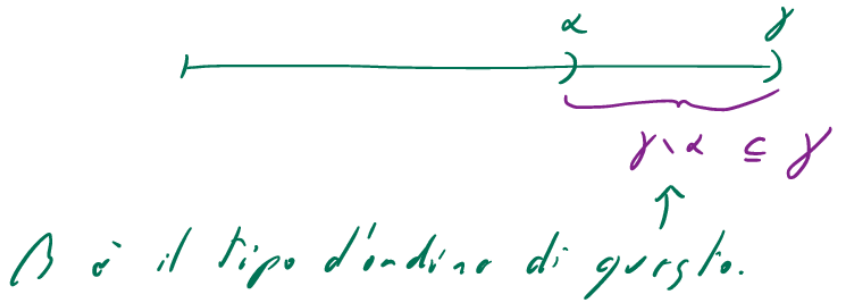
\includegraphics[width = 6.0cm]{immagini/sottrazione_ordinali.png}
\end{figure}

\textcolor{MidnightBlue}{Vediamo ora una dimostrazione formale.}

\begin{proof}
	Vediamo esistenza e unicità separatamente.
	\begin{itemize}
		\item[$\boxed{\text{unicità}}$] Abbiamo l'unicità perché la funzione $+$ è strettamente crescente nel secondo argomento, come visto in precedenza, dunque se ci fosse un altro ordinale diverso da $\beta$, per la totalità dell'ordinamento sugli
		ordinali, sarebbe $<$ o $>$ di $\beta$, da cui anche la somma sarebbe strettamente minore o maggiore e quindi diversa da $\gamma$, pertanto $\beta$ è unico.
		\item[$\boxed{\text{esistenza}}$] Se $\alpha = \gamma$ è sufficiente prendere $\beta = 0$. Possiamo quindi supporre che $\alpha < \gamma$ e consideriamo
		il minimo $\delta$ tale che la somma supera $\gamma$, $\gamma < \alpha + \delta$ - $\delta$ esiste poiché $\gamma \;\textcolor{red}{<}\; s(\gamma) \leq \alpha + s(\gamma)$ e quindi l'insieme degli ordinali la cui somma con $\alpha$ a sinistra è maggiore strettamente di $\gamma$ è non vuoto.\\
		Se $\delta$ è successore, $\delta = \beta + 1$, allora, per la minimalità di $\delta$, si ha $\alpha + \beta \leq \gamma < s(\alpha + \beta) = \alpha + s(\beta) = \alpha + \delta$, pertanto nella prima disuguaglianza non può valere il minore stretto, perché se così fosse si avrebbe che $\gamma \geq s(\alpha + \beta) = \alpha + \delta$, che è assurdo, 
		quindi abbiamo proprio che $\alpha + \beta = \gamma$.\\
		Osserviamo ora che $\delta$ non non può essere limite e così abbiamo concluso. Se $\delta$ fosse limite avremmo:
		\[ \gamma \overset{\text{def. $\delta$}}{<} \alpha + \delta \overset{\text{def. +}}{=} \sup_{\varepsilon < \delta}(\alpha + \varepsilon)
			\] 
		ma allora, dovendo essere il sup di un insieme non vuoto, ciò vuol dire, affinché la disuguaglianza scritta sia vera, che esiste $\varepsilon < \delta$ tale che $\gamma < \alpha + \varepsilon$, contro la minimalità di $\delta$, che è assurdo. Alternativamente,
		ci bastava osservare che, per la minimalità di $\delta$, $\alpha + \varepsilon \leq \gamma$, per ogni $\varepsilon < \delta$, per cui passando la disuguaglianza al sup, avremmo ottenuto $\sup_{\varepsilon < \delta}(\alpha + \varepsilon) \leq \gamma$, che unito alla catena sopra ci dà ancora una volta un assurdo.\footnote{Il passaggio delle disuguaglianze larghe al sup è conseguenza del lemma visto ad inizio capitolo sulle disuguaglianze tra sup.}\,\footnote{L'esistenza può essere dimostrata in modo equivalente per induzione transfinita.}
	\end{itemize}
\end{proof}

\pagebreak

\begin{lemma}[Divisione euclidea di ordinali]
	Dati $\alpha,\gamma \in \Ord$, con $\alpha \ne 0$, esistono e \textcolor{red}{sono unici} $\beta, \rho \in \Ord$ tali che $\rho < \alpha$ e $\alpha \cdot \beta + \rho = \gamma$.
\end{lemma}

\begin{proof}
	Verifichiamo esistenza e unicità separatamente.
	\begin{itemize}
		\item[$\boxed{\text{unicità}}$] Fissato $\beta$, $\rho$ è unico, o per monotonia stretta nella seconda componente della somma o per il lemma sulla sottrazione visto sopra\footnote{Di fatto, essendo che l'unicità nella sottrazione la si ha come conseguenza della monotonia stretta nella seconda componente, il motivo per cui si ha unicità è sempre la monotonia della somma.}.
		Dobbiamo quindi dimostrare solo l'unicità di $\beta$. Supponiamo per assurdo di avere $\beta \ne \beta'$, e WLOG $\beta < \beta'$, con relativamente resti $\rho,\rho' < \alpha$, per cui $\alpha \cdot \beta + \rho = \alpha \cdot \beta' + \rho'$, allora sfruttando la monotonia si ottiene:
		\begin{align*}
			\alpha \cdot \beta +\rho  & \;\textcolor{red}{<}\; \alpha \cdot \beta + \alpha \\
									  & = \alpha \cdot s(\beta) &&\text{(def. ricorsiva $\cdot$)} \\
									  & \leq \alpha \cdot \beta' &&(\beta < \beta')\\
									  & \leq \alpha \cdot \beta' + \rho' &&(\rho' \geq 0)\\
									  & = \alpha \cdot \beta + \rho \quad \textcolor{red}{\lightning} &&(\text{Hp. assurda})
		\end{align*}
		\item[$\boxed{\text{esistenza}}$] Procediamo come nella dimostrazione del lemma di sottrazione, e consideriamo il minimo $\delta$ tale che $\gamma < \alpha \cdot \delta$ - tale $\delta$ esiste, cioè l'insieme è non vuoto, in quanto $\gamma = 1 \cdot \gamma \leq \alpha \cdot \gamma < \alpha \cdot s(\gamma)$.
		Assumiamo che $\delta$ sia successore, $\delta = s(\beta)$, allora per la minimalità di $\delta$, si ha $\alpha \cdot \beta \leq \gamma$\footnote{Notare che non vale necessariamente l'uguale come nella dimostrazione del lemma di sottrazione perché, supponendo il minore stretto, qui avremmo
		$\gamma \geq s(\alpha \cdot \beta) \ne \alpha \cdot \beta + \beta =  \alpha \cdot s(\beta) =\alpha \cdot \delta$.}, possiamo quindi applicare il lemma di sottrazione ordinale ed ottenere l'unico $\rho$ per cui:
		\[ \alpha \cdot \beta + \rho = \gamma
			\]
		Osserviamo ora che $\rho < \alpha$, infatti, se per assurdo fosse $\rho \geq \alpha$, avremmo:
		\begin{align*}
			\gamma & \;\textcolor{red}{<} \; \alpha \cdot \delta \\
				   & = \alpha \cdot s(\beta) \\
				   & = \alpha \cdot \beta + \alpha \\
				   & \leq \alpha \cdot \beta + \rho = \gamma \quad \textcolor{red}{\lightning}
		\end{align*}
		Infine dobbiamo verificare che $\delta$ non sia limite, se per assurdo lo fosse, avremmo:
		\[ \gamma < \alpha \cdot \delta = \sup_{\varepsilon < \delta} (\alpha \cdot \varepsilon)
			\]
		dove, affinché la disuguaglianza sia valida, il sup al RHS deve essere ben definito, e per un insieme di ordinali lo è, come abbiamo visto, quando l'insieme è non vuoto,
		per cui esiste $\varepsilon < \delta$ tale per cui $\gamma < \alpha \cdot \varepsilon$, contro la minimalità di $\delta$, che è assurdo.\\
		Alternativamente si può osservare che, per la minimalità di $\delta$, $\forall \varepsilon < \delta \; \alpha \cdot \varepsilon \leq \gamma$, tale disuguaglianza passa al sup,
		ed aggiunta in fondo alla catena scritta sopra ci dà nuovamente un assurdo.
	\end{itemize}
\end{proof}

\subsection{La forma normale di Cantor}

\begin{theorem}[Forma normale di Cantor - CNF]
	Ogni ordinale $\alpha$ può essere espresso in maniera unica come somma \textcolor{red}{finita} del tipo:
	\[ \alpha = \omega^{\beta_1} \cdot k_1 + \omega^{\beta_2} \cdot k_2 + \ldots + \omega^{\beta_n} \cdot k_n
		\]
	con $\beta_1 > \beta_2 > \ldots > \beta_n$ ordinali, $k_1,k_2,\ldots,k_n \in \omega\setminus\{0\}$ e $n \in \omega$.
\end{theorem}

\begin{proof}
	Dividiamo la dimostrazione in esistenza ed unicità.
	\begin{itemize}
		\item[$\boxed{\text{esistenza}}$] Procediamo per induzione transfinita, supponiamo che ogni ordinale strettamente più piccolo di $\alpha$ abbia una forma normale e verifichiamo che anche $\alpha$ la abbia.\\
		Sia $\gamma$ il minimo tale che $\alpha < \omega^\gamma$ - che esiste in quanto $\alpha \leq \omega_\alpha < \omega^{s(\alpha)}$, dove la prima disuguaglianza è il fatto che $x \mapsto \omega^x$ è una funzione strettamente crescente tra buoni ordini.
		Come nei lemmi precedenti, diamo per buono che $\gamma$ sia successore, $\gamma = s(\beta)$, allora abbiamo che $\omega^\beta \leq \alpha$, possiamo fare la divisione euclidea di $\alpha$ per $\omega^\beta$ e ottenere:
		\[ \alpha = \omega^\beta \cdot k + \rho \qquad \rho < \omega^\beta \leq \alpha
			\]
		con $k$ e $\rho$ unici. A questo punto vale l'ipotesi induttiva per $\rho$ e lo si può scrivere in CNF, per verificare che allora anche $\alpha$ sia scritto in CNF è necessario osservare due cose. In primis che $0 < k < \omega$, infatti:
		\begin{itemize}
			\item \textbf{\underline{$k = 0$}}: in questo caso $\alpha = \rho < \alpha \; \lightning$.
			\item \textbf{\underline{$k \geq \omega$}}: in questo caso $\alpha \;\textcolor{red}<\;\omega^\gamma = \omega^{s(\beta)} = \omega^\beta \cdot \omega \leq \omega^\beta \cdot k \leq \omega^\beta \cdot k + \rho = \alpha \; \lightning$.
		\end{itemize}
		Osserviamo inoltre che, dato che $\rho < \omega^\beta$, scrivendo, con l'ipotesi induttiva, $\rho = \omega^{\beta_2} \cdot k_2 + \ldots + \omega^{\beta_n} \cdot k_n$, si ha $\beta_2 < \beta$, infatti, se così non fosse, cioè se fosse che $\beta_2 \geq \beta$, avremmo:
		\[ \omega^\beta \leq \omega^{\beta_2} \leq \omega^{\beta_2} \cdot k_2 + \ldots + \omega^{\beta_n} \cdot k_n = \rho \;\textcolor{red}<\; \omega^\beta \; \textcolor{red}\lightning
			\]
		pertanto la scrittura ottenuta dalla divisione di $\alpha$ per $\omega^\beta$ è effettivamente una scrittura di $\alpha$ in forma normale di Cantor.\\
		Ci resta soltanto da verificare che il $\gamma$ usato all'inizio non è limite, se per assurdo lo fosse, avremmo:
		\[ \alpha < \omega^\gamma = \sup_{\delta < \gamma} \omega^\delta
			\]
		e affinché la disuguaglianza sia vera il sup al RHS deve essere ben definito, e lo è a condizione che l'insieme di ordinali su cui è preso è non vuoto, ovvero a condizione che esista $\delta < \gamma$ tale che $\alpha < \omega^\delta$, contro la minimalità di $\gamma$.\footnote{Come al
		solito si può osservare alternativamente anche che la disuguaglianza $\omega^\delta \leq \alpha$, valida per la minimalità di $\gamma$, passa al sup generando ancora una volta un assurdo.}
		\item[$\boxed{\text{unicità}}$] Sia $\alpha$ minimo ordinale che non ha un'unica forma normale\footnote{Lo possiamo prendere perché abbiamo visto che la classe degli ordinali è bene ordinata.}, per cui abbiamo che $\alpha$ si può scrivere in almeno due forme normali di Cantor distinte:
		\[ \begin{split}
			\alpha &= \omega^{\beta_1} \cdot k_1 + \omega^{\beta_2} \cdot k_2 + \ldots + \omega^{\beta_n} \cdot k_n \\
				   &= \omega^{\beta_1'} \cdot k_1' + \omega^{\beta_2'} \cdot k_2' + \ldots + \omega^{\beta_{n'}'} \cdot k_{n'}'
		\end{split}
			\]
		dove $n'$ non è necessariamente uguale ad $n$, per cui le scritture possono avere lunghezza diversa.
		Ci basta dimostrare che $\beta_1 = \beta_1'$ e $k_1 = k_1'$, infatti in tal caso, per la stretta monotonia otteniamo:
		\[ \omega^{\beta_2} \cdot k_2 + \ldots + \omega^{\beta_n} \cdot k_n = \omega^{\beta_2'} \cdot k_2' + \ldots + \omega^{\beta_{n'}'} \cdot k_{n'}' \;\textcolor{purple}{<\;\omega^{\beta_1},\omega^{\beta_1'}} 
			\]
		dunque avremmo trovato un ordinale strettamente più piccolo di $\alpha$ con almeno due scritture distinte in CNF e quindi avremmo un assurdo.\\
		Se abbiamo che $\beta_1 = \beta_1'$, allora necessariamente anche $k_1 = k_1'$, infatti in questo caso possiamo scrivere:
		\[ \alpha = \omega^{\beta_1} \cdot k_1 + \underbrace{\ldots}_{\textcolor{purple}{< \omega^{\beta_1}}} = \omega^{\beta_1} \cdot k_1' + \underbrace{\ldots}_{\textcolor{purple}{< \omega^{\beta_1}}}
			\]
		cioè nella forma della divisione euclidea, e quindi otteniamo $k_1 = k_1'$, per unicità della scrittura in questa forma\footnote{Inoltre otterremo anche che le code sono uguali, ma di nuovo ciò è di fatto sempre una conseguenza della monotonia stretta sulla seconda componente.}.\\
		Ci resta quindi solo da verificare che $\beta_1 = \beta_1'$, se per assurdo supponessimo, WLOG, che $\beta_1 < \beta_1'$, dunque $s(\beta_1) \leq \beta_1'$, avremmo:
		\[ \alpha = \omega^{\beta_1} \cdot k_1 + \omega^{\beta_2} \cdot k_2 + \ldots + \omega^{\beta_n} \cdot k_n \; \textcolor{purple}{<\; \omega^{s(\beta_1)}} \leq \omega^{\beta_1'} \cdot k_1' + \ldots = \alpha \; \textcolor{red}\lightning
			\]
	\end{itemize}
\end{proof}

\begin{exercise}
	Dimostrare le disuguaglianza in \textcolor{purple}{viola} (sono tutte uguali).
\end{exercise}

\begin{soln}
	Per l'ultima disuguaglianza basta osservare che per monotonia:
	\[ \omega^{\beta_1} \cdot k_1 + \omega^{\beta_2} \cdot k_2 + \ldots + \omega^{\beta_n} \cdot k_n \leq \omega^{\beta_1} \cdot k_1 + \omega^{\beta_{\textcolor{red}1}} \cdot k_2 + \ldots + \omega^{\beta_{\textcolor{red}1}} \cdot k_n = \omega^{\beta_1} \cdot (\underbrace{k_1 + \ldots + k_n}_{=: k})
		\]
	e a questo punto $\omega^{\beta_1} \cdot k \;\textcolor{red}{<}\; \omega^{\beta_1} \cdot \omega = \omega^{s(\beta_1)}$. Per le prime tre disuguaglianze, basta ragionare in maniera identica con $\omega^{\beta_2} \cdot k_2 + \ldots + \omega^{\beta_n} \cdot k_n$ (analogamente con la versione con i $'$), ottenendo
	$\omega^{\beta_2} \cdot k \;\textcolor{red}{<}\; \omega^{\beta_2} \cdot (k + 1) \leq \omega^{s(\beta_2)} \leq \omega^{\beta_1}$.
\end{soln}

\subsection{Punti fissi e \texorpdfstring{$\varepsilon$}{epsilon}-numbers}
Si potrebbe credere che il teorema precedente, applicato ricorsivamente agli esponenti $\beta_1,\ldots,\beta_n$, implichi che ogni ordinale
si possa scrivere sotto forma di un'espressione finita composta di somme, prodotti e potenze delle costanti $0,1,2,\ldots,\omega$. Tipo questa:
\[ \omega^{\omega^4 \cdot 7 + \omega^2 \cdot 1}\cdot 9 + \omega^{75} + 9
	\]
Effettivamente, se valesse $\textcolor{red}{\alpha > \beta_1}>\beta_2>\ldots>\beta_n$ per ogni $\alpha$, allora questa conclusione sarebbe corretta.
Però è possibile esibire un ordinale $\varepsilon_0$ - e, in realtà, un'intera classe propria di ordinali come questo - tale che $\varepsilon_0 = \omega^{\varepsilon_0}$\footnote{Notare che in questo caso non vale che $\alpha > \beta_1$, e quindi $\varepsilon_0$ non può essere scritto nella forma sopra.}.
La forma normale di Cantor di $\varepsilon_0$ è quindi, chiaramente, $\omega^{\varepsilon_0}$, e procedere ricorsivamente sull'esponente $\omega^{\omega^{\varepsilon_0}},\omega^{\omega^{\omega^{\varepsilon_0}}}$, etc. non conduce ad un'espressione finita, intuitivamente verrebbe una cosa del tipo:
\[ \varepsilon_0 = \underbrace{\omega^{\omega^{\omega^{\omega^{\iddots}}}}}_{\text{$\omega$ volte}}
	\]
La proposizione seguente è interessante di per sé, ma, in particolare, ci permetterà di dimostrare l'esistenza degli \vocab{$\varepsilon$-numbers}.

\begin{proposition}[Ogni funzione normale ha una classe propria di punti fissi]
	Sia $F : \Ord \rightarrow \Ord$ una funzione classe \textcolor{orange}{strettamente} crescente e continua\footnote{Tali funzioni prendono il nome di \vocab{funzioni normali.}} - ossia $F(\lambda) = \sup F[\lambda] = \sup_{\alpha < \lambda} F(\alpha)$ per $\lambda$ limite.
	Allora, per ogni $\alpha \in \Ord$, $F$ ha un punto fisso $\geq \alpha$, ossia vale che:
	\[ \exists \pi \in \Ord \; \alpha \leq \pi \land F(\pi) = \pi
		\]
\end{proposition}

\begin{proof}
	Fissato $\alpha \in \Ord$ costruiamo un punto fisso di $F$ che sia maggiore o uguale ad $\alpha$. Definiamo per ricorsione numerabile:
	\[ \pi_n := \begin{cases}
		\pi_0 = \alpha \\
		\pi_{n+1} = F(\pi_n)
	\end{cases}
		\]
	se $F(\alpha) = \alpha$ allora $\pi_n = \alpha$ ed abbiamo il punto fisso voluto, altrimenti, essendo $F$ strettamente crescente, si ha $\alpha < F(\alpha)$, cioè $\pi_0 < \pi_1$\footnote{Typo Mamino scrive ovunque 0 al posto di $\alpha$.}, da cui si verifica per induzione che $\pi_n$ è
	strettamente crescente\footnote{Per ipotesi induttiva $\pi_{n-1} < \pi_n$, e poiché $F$ è strettamente crescente, applicandola alla disuguaglianza si ottiene $\pi_n < \pi_{n+1}$, quindi il passo induttivo.}, $\forall n \in \omega \; \pi_n < \pi_{n+1}$, di conseguenza, detto:
	\[ \pi \Mydef \sup_{n \in \omega} \pi_n
		\]
	abbiamo che $\pi$ è un ordinale limite, poiché $\pi \not \in \{\pi_n | n \in \omega\}$ (altrimenti non sarebbe il sup), inoltre naturalmente $\pi > \pi_0 = \alpha$, per cui:
	\[ F(\pi) \overset{\text{$F$ continua}}{=} \sup_{n \in \omega} F(\pi_n) \overset{\text{def}}{=} \sup_{n \in \omega} \pi_{n+1} = \pi
		\]
\end{proof}

\begin{remark}[I punti fissi sono una classe propria di ordinali]
	Abbiamo dimostrato che per ogni ordinale c'è un punto fisso di $F$ (sotto opportune ipotesi) che è maggiore di tale ordinale, pertanto i punti fissi di $F$ non possono formare un insieme di ordinali perché non esiste un estremo superiore,
	dunque formano una (sotto)classe propria di $\Ord$.
\end{remark}

\begin{example}[$x \mapsto \omega^x$]
	La mappa $x \mapsto \omega^x$ è strettamente crescente, per la monotonia stretta dell'esponenziale nella seconda componente, ed è continua in quanto abbiamo definito l'esponenziale di ordinali infiniti estendendo per continuità la definizione dal caso finito,
	pertanto per il teorema sopra tale mappa ha una classe propria di punti fissi, che sono appunto tali per cui $\varepsilon = \omega^{\varepsilon}$.
\end{example}

\begin{exercise}
	Sia $\varepsilon_0 = \sup\{1,\omega,\omega^{\omega},\omega^{\omega^{\omega}}, \omega^{\omega^{\omega^{\omega}}},\ldots\}$. Formalmente definiamo per ricorsione numerabile $\alpha_0 = 1$, $\alpha_{n+1}=\omega^{\alpha_n}$,
	allora $\varepsilon_0 = \sup\{\alpha_n | n \in \omega\}$. Dimostrare che $\varepsilon_0$ è il più piccolo punto fisso della funzione $x \mapsto \omega^x$.
\end{exercise}

\begin{soln}
	Osserviamo in primis che $\varepsilon_0$ è un ordinale limite, per farlo ci basta osservare che $\varepsilon_0 \not \in \{\alpha_n | n \in \omega\}$, infatti la successione $\alpha_n$ è strettamente crescente, dunque se fosse che $\varepsilon_0 = \alpha_m$, per $m \in \omega$,
	allora $\alpha_{m+1} > \varepsilon_0$ e quindi quest'ultimo non sarebbe il sup, che è assurdo, segue quindi che $\varepsilon_0$ è limite per un lemma visto.\footnote{In realtà non serve osservarlo per poter applicare il lemma di commutazione tra potenze e sup di insiemi di ordinali, ma è comunque interessante notarlo.}\\
	Verifichiamo ora che $\varepsilon_0$ è un punto fisso di $x \mapsto \omega^x$:
	\[ \varepsilon_0 \overset{\text{def.}}{=} \sup_{n \in \omega} \alpha_n \overset{(\star)}{=} \sup_{n \in \omega} \omega^{\alpha_n} \overset{\text{lemma}}{=} \omega^{\sup_{n \in \omega} \alpha_n} \overset{\text{def.}}{=} \omega^{\varepsilon_0}
		\]
	dove $(\star)$ vale per il lemma della disuguaglianza dei sup applicato in ambo i versi, infatti dato $\alpha_n$, è sufficiente prendere $\omega^{\alpha_n}$ nel secondo insieme per avere la prima disuguaglianza, viceversa, preso $\omega^{\alpha_n}$ nel secondo, basta osservare che $\alpha_{n+1} = \omega^{\alpha_n}$ è nel primo.\\
	Infine osserviamo che $\varepsilon_0$ è il più piccolo punto fisso di $x \mapsto \omega^x$, infatti, se esistesse $y < \varepsilon_0$ punto fisso di $x \mapsto \omega^x$, allora avremmo:
	\[ \alpha_n \leq y < \alpha_{n+1}\,\footnote{Il caso $y \in \omega$ andrebbe fatto a parte per essere precisi, ma è molto facile osservare che anche in questo caso segue la tesi.}
		\]
	infatti $y \in \bigcup_{n+1}\alpha_n$, dunque $y$ è almeno in un $\alpha_n$ che è successore (altrimenti basta prendere il successivo), e ci basta prendere il minimo successore a cui appartiene per avere la disuguaglianza sopra (se il termine di testa di $y$ in CNF non fosse $\geq \alpha_n$, allora $\alpha_{n+1}$ non sarebbe il minimo a cui appartiene $y$).
	Dalle disuguaglianze sopra segue che:
	\[ \alpha_{n+1} = \omega^{\alpha_n} \leq \omega^y \leq \omega^{\alpha_{n+1}} = \alpha_{n+2}
		\]
	per cui se $y$ fosse un punto fisso, si avrebbe $y < \alpha_{n+1} \leq \omega^y = y \; \lightning$.
\end{soln}

\begin{exercise}[Lista dei punti fissi di una funzione normale]
	Sia $F : \Ord \rightarrow \Ord$ crescente e continua, allora esiste $G : \Ord \rightarrow \Ord$ strettamente crescente tale che:
	\[ \forall \alpha \in \Ord \; F(\alpha) = \alpha \leftrightarrow \exists \beta \in \Ord \; \alpha = G(\beta)
		\]
\end{exercise}

\begin{soln}
	Dalla proposizione sopra abbiamo visto che i punti fissi di $F : \Ord \to \Ord$ sono una classe propria $C_F$, dunque possiamo definire per ricorsione transfinita:
	\[ G(\alpha) = \min\{x \in C_F : \forall y \in G[\alpha] \; x > y\}\,\footnote{Non stiamo usando separazione, è solo una formula insiemistica, e il minimo è sempre ben definito perché la classe $C_F$ è una sottoclasse di $\Ord$ che è bene ordinata, e $C_F$ è sempre non vuota perché è una classe propria.}
		\]
	che è ben definita per il teorema di ricorsione transfinita, ed è strettamente crescente per costruzione. Verifichiamo inoltre che $\Imm(G) = C_F$, preso $\beta \in C_F$, si ha che:
	\[ \beta < s(\beta) \leq G(s(\beta))
		\]
	ed essendo $G(s(\beta))$ il più piccolo ordinale in $C$ più grande di tutti gli ordinali di $G[s(\beta)]$, per minimalità, si ha che esiste $\gamma \in G[s(\beta)]$ tale che $\gamma \geq \beta$, da cui $\beta \in G[s(\beta)]$, e quindi $\beta \in \Imm(G)$.
	Segue quindi che $G$ è un isomorfismo tra $\Ord$ e $C_F \subseteq \Ord$, ed in tal modo soddisfa la tesi, infatti $\forall \alpha \in \Ord \; F(\alpha) = \alpha \iff \alpha \in C_F \overset{\text{$G$ surg.}}{\iff} \exists \beta \in C_F \; G(\beta) = \alpha$.
\end{soln}

\begin{exercise}[Unicità della lista]
	La $G$ dell'esercizio precedente è univocamente determinata da $F$ ed è una funzione classe continua.
\end{exercise}

\begin{soln}
	Verifichiamo che data $H : \Ord \to C_F \subseteq \Ord$ strettamente crescente e che soddisfi la proprietà $\forall \alpha \in \Ord \; F(\alpha) = \alpha \leftrightarrow \exists \beta \in \Ord \; \alpha = H(\beta)$ (che equivale al fatto che $\Imm(H) = C_F$,
	ovvero $H$ isomorfismo tra $\Ord$ e $C_F$, la classe propria dei punti fissi di $F$), allora soddisfa la definizione ricorsiva di $G$ data nell'esercizio precedente,
	e quindi coincide proprio con quest'ultima per il teorema di ricorsione transfinita, da cui segue quindi l'unicità della lista dei punti fissi $G$.\\
	Poiché $H$ è strettamente crescente per ipotesi, naturalmente $H(\alpha)$ è più grande di tutti gli elementi di $H[\alpha]$, inoltre,
	se esistesse $\gamma \in C_F$, tale che $\gamma < H(\alpha)$ e maggiore di tutti gli $H[\alpha]$, allora $\gamma > F(\delta)$ per $\delta < \alpha$, per la monotonia di $H$, e $\gamma < F(\delta)$ per $\delta \geq \alpha$, dunque $\gamma \not\in \Imm(H)$, che è per ipotesi contro la surgettività di $H : \Ord \to C_F$,
	dunque $H(\alpha)$ è proprio il più piccolo ordinale di $C_F$ più grande di tutti gli ordinali in $H[\alpha]$, pertanto $H$ soddisfa la relazione ricorsiva di $G$ e quindi coincide con quest'ultima.\\
	La continuità di $G$ segue banalmente dalla definizione ricorsiva che abbiamo dato, infatti:
	\[ G(\lambda) = \min\{x \in C_F : \forall y \in G[\lambda] \; x > y\} = \sup G[\lambda] = \sup_{\alpha < \lambda} G(\alpha)
		\]
\end{soln}

\begin{remark}[Derivata di funzioni ordinali]
	Data una funzione $F : \Ord \to \Ord$ normale la proposizione iniziale ci dice che $F$ ha una classe propria di punti fissi, e gli ultimi due esercizi ci dicono che tali punti fissi possono essere elencata in modo unico e strettamente crescente da una nuova funzione $G : \Ord \to \Ord : \alpha \mapsto \alpha$-esimo punto fisso di $F$,
	tale funzione prende talvolta in letteratura il nome di \vocab{derivata} di $F$. Notare infine che $G$, per quanto abbiamo visto, è, per costruzione, a sua volta normale, dunque può essere ``derivata'' a sua volta, dandoci nuovamente un'unica lista dei suoi punti fissi.
\end{remark}

\begin{definition}[$\varepsilon$-numbers]
	Definiamo l'unica funzione che elenca i punti fissi di $x \mapsto \omega^x$, ovvero la sua derivata, $\varepsilon_\alpha$, i cui valori prendono il nome di \vocab{epsilon-numbers} e sono appunto i punti fissi di $x \mapsto \omega^x$ elencati in maniera ordinata dagli ordinali.
\end{definition}

\begin{definition}[$\zeta$-numbers]
	Definiamo l'unica funzione che elenca i punti fissi della funzione $\varepsilon_\alpha$, ovvero la sua derivata\footnote{Sarebbe la derivata seconda di $x \mapsto \omega^x$.}, $\zeta_\alpha$, i cui valori prendono il nome di \vocab{zeta-numbers} e sono appunto i punti fissi di $\zeta_\alpha$ elencati in maniera ordinata dagli ordinali.
\end{definition}

I primi due esercizi seguenti saranno assai più facili quando, usando l'assioma della scelta, dimostreremo che un insieme numerabile di insiemi numerabili è numerabile.\footnote{Ricordare che l'avevamo già dimostrato dando per buono di avere una successione di enumerazioni,
ma anche il quel caso l'enumerazione ce la si può procurare solo con scelta.}

\begin{exercise}[\textcolor{red}{$\star$ Difficile senza leggere l'idea sotto}]
	$|\varepsilon_0| = \aleph_0$.\footnote{\underline{\textbf{Idea}}: dimostrare che $\alpha \in \varepsilon_0$ se e solo se $\alpha$ può essere scritto a partire da $0,1,\omega$, applicando le operazioni di somma, prodotto, ed esponente ordinale un numero finito di volte.}
\end{exercise}

\begin{soln}
	Per definizione $\varepsilon_0 = \sup\{\alpha_n | n \in \omega\}$, dove $\alpha_0 = 1$ e $\alpha_{n+1}=\omega^{\alpha_n}$, si ha che $\varepsilon_0 \geq \alpha_1 = \omega$, dunque $\omega \subseteq \varepsilon_0 \to \aleph_0 \leq |\varepsilon_0|$.\footnote{Se avessimo AC
	potremmo concludere immediatamente l'altra disuguaglianza dimostrando per induzione che $|\alpha_n| = \aleph_0$, da cui $|\varepsilon_0| = |\sup_{n \in \omega} \alpha_n| = |\bigcup_{n \in \omega} \alpha_n| \overset{\text{AC}}{\leq} \aleph_0$.} Per la
	disuguaglianza opposta
\end{soln}

\begin{exercise}[\textcolor{red}{$\star \star$ Ostico}]
	Sia $\zeta_0$ minimo tale che $\varepsilon_{\zeta_0} = \zeta_0$, allora $|\zeta_0| = \aleph_0$.
\end{exercise}

\begin{soln}
	Per gli esercizi sopra, sappiamo che $\zeta_\alpha$ è la funzione che elenca i punti fissi di $\varepsilon_\alpha$ in maniera strettamente crescente, dunque $\zeta_0$ è il più piccolo punto fisso di $\varepsilon_\alpha$ per definizione.
	Dallo stesso teorema, sappiamo che $\varepsilon_\alpha$, essendo a sua volta successione crescente di punti fissi di $x \mapsto \omega^x$, è strettamente crescente, per cui $\varepsilon_0 \leq \varepsilon_{\zeta_0}$, da cui otteniamo la disuguaglianza dal basso $\aleph_0 = |\varepsilon_0| \leq |\varepsilon_{\zeta_0}|$.\\
	Per il viceversa
\end{soln}

\begin{exercise}[Teorema di scrittura in base ordinale]
	Sia $\gamma$ un qualunque ordinale $\geq 2$. Ogni ordinale $\alpha$ si scrive in modo unico come somma finita:
	\[ \alpha = \gamma^{\beta_1}\cdot k_1 + \ldots \gamma^{\beta_n}\cdot k_n
		\]
	con $\beta_1 > \beta_2 > \ldots > \beta_n$ ordinali, $k_1,\ldots,k_n \in \gamma\setminus\{0\}$ e $n \in \omega$.
\end{exercise}

\begin{soln}
	Dividiamo esistenza ed unicità della scrittura in base $\gamma$.
	\begin{itemize}
		\item[$\boxed{\text{esistenza}}$] Procediamo per induzione transfinita forte, dunque supponiamo che tutti gli ordinali minori strettamente di $\alpha$ si possano scrivere in base $\gamma$ come sopra, e dimostriamo che anche $\alpha$ si può scrivere in tale forma.\\
		Sia $\delta$ il minimo ordinale tale che $\alpha < \gamma^\delta$ - che esiste in quanto $x \mapsto \gamma^x$ è strettamente crescente tra classi bene ordinate, per cui $\alpha \leq \gamma^\alpha < \gamma^{s(\alpha)}$, e quindi la sottoclasse di $\Ord$ da cui prendiamo il minimo è non vuota.
		Assumiamo che $\delta = \beta + 1$, e per minimalità di $\delta$ si ha $\gamma^\beta \leq \alpha$ e applichiamo il lemma di divisione euclidea per ottenere:
		\[ \alpha = \gamma^\beta \cdot k + \rho \qquad \rho < \gamma^\beta \leq \alpha
			\]
		con $k$ e $\rho$ unici. Possiamo applicare l'ipotesi induttiva a $\rho$ e scrivere $\rho = \gamma^{\beta_2}\cdot k_2 + \ldots + \gamma^{\beta_n} \cdot k_n$, a questo punto, per dire che la scrittura trovata dalla divisione sostituendo $\rho$ con la sua scrittura in base $\gamma$,
		è effettivamente una scrittura in base $\gamma$ per $\alpha$, dobbiamo verificare due cose. In primis osserviamo che $0 < k < \gamma$:
		\begin{itemize}
			\item \underline{$k = 0$}: in tal caso $\alpha = \rho < \alpha \; \textcolor{red}\lightning$.
			\item \underline{$k \geq \gamma$}: in questo caso $\gamma^\delta = \gamma^{\beta + 1} = \gamma^\beta \cdot \gamma \leq \gamma^\beta \cdot k \leq \gamma^\beta \cdot k + \rho = \alpha \;\textcolor{red}<\; \gamma^\delta \; \textcolor{red}\lightning$. 
		\end{itemize}
		Osserviamo inoltre che $\beta > \beta_2$, infatti, se fosse $\beta_2 \geq \beta$ si avrebbe:
		\[ \gamma^\beta \leq \gamma^{\beta_2} \leq \gamma^{\beta_2} \cdot k_2 + \ldots + \gamma^{\beta_n} \cdot k_n = \rho \;\textcolor{red}<\; \gamma^{\beta} \quad \textcolor{red}\lightning
			\]
		quindi abbiamo ottenuto che esiste almeno una scrittura in base $\gamma$ per $\alpha$. Ci resta soltanto da verificare l'assunzione iniziale che $\delta$ sia successore e non limite, se $\delta$ fosse limite si avrebbe:
		\[ \alpha < \gamma^\delta = \sup_{\varepsilon < \delta} \gamma^{\varepsilon}
			\]
		affinché la disuguaglianza sia vera l'insieme di ordinali su cui si prende il sup al RHS deve essere non vuoto, cioè deve esistere $\varepsilon < \delta$ tale che $\alpha < \gamma^{\varepsilon}$, contro la minimalità di $\delta$. Alternativamente
		si può osservare che, per la minimalità di $\delta$, si ha $\forall \varepsilon < \delta \; \gamma^{\varepsilon} \leq \alpha$, e, passando questa disuguaglianza al sup - cosa che si può fare per il lemma sulla disuguaglianza dei sup - si ottiene $\gamma^\delta = \sup_{\varepsilon < \delta} \gamma^{\varepsilon} \leq \alpha \; \textcolor{red}\lightning$.
		\item[$\boxed{\text{unicità}}$] Sia $\alpha$ il minimo ordinale che non si scrive in modo unico in base $\gamma$ - se la sottoclasse di tali ordinali fosse vuota avremmo già la tesi - ovvero:
		\begin{align*}
			\alpha &= \gamma^{\beta_1}\cdot k_1 + \ldots \gamma^{\beta_n}\cdot k_n \\
				   &= \gamma^{\beta_1'}\cdot k_1' + \ldots \gamma^{\beta_n'}\cdot k_n'
		\end{align*}
		Osserviamo che se $\beta_1 = \beta_1'$ e $k_1 = k_1'$, allora per la stretta monotonia della somma sulla seconda componente si ottiene:
		\[ \gamma^{\beta_2}\cdot k_2 + \ldots \gamma^{\beta_n}\cdot k_n = \gamma^{\beta_2}\cdot k_2 + \ldots \gamma^{\beta_n}\cdot k_n < \alpha
			\]
		ovvero che esiste un ordinale più piccolo di $\alpha$ che ammette due scritture in base $\gamma$, contro la minimalità di $\alpha$. Osserviamo inoltre che se $\beta_1 = \beta_1'$,
		allora necessariamente $k_1 = k_1'$, infatti:
		\[ \alpha = \gamma^{\beta_1}\cdot k_1 + \underbrace{\ldots}_{<\gamma^{\beta_1}} = \gamma^{\beta_1'} \cdot k_1' + \underbrace{\ldots}_{<\gamma^{\beta_1'}} 
			\]
		dunque $k_1 = k_1'$ e c'è uguaglianza delle code per unicità data dal lemma di divisione.
		Verifichiamo infine che necessariamente $\beta_1 = \beta_1 '$, infatti, se fosse WLOG $\beta_1 < \beta_1'$, cioè si avrebbe:
		\[ \alpha = \gamma^{\beta_1}\cdot k_1 + \ldots \gamma^{\beta_n}\cdot k_n \leq \gamma^{\beta_1} \cdot k \;\overset{\textcolor{purple}{k < \gamma}}{<}\; \gamma^{s(\beta_1)} \leq \gamma^{\beta_1 '} \leq \gamma^{\beta_1'}\cdot k_1' + \ldots \gamma^{\beta_n'}\cdot k_n' = \alpha \; \textcolor{red}\lightning
			\]
		dove abbiamo posto $k = k_1 + \ldots + k_n$.
	\end{itemize}
\end{soln}

\subsection{Operazioni in forma normale di Cantor}
È facile ridurre l'aritmetica ordinale, in forma normale di Cantor, ad una piccola collezione di regole meccaniche.
Nel contesto del corso, queste regole hanno un'importanza limitata, è però utile sapere che ci sono, ed avere un'idea del loro aspetto.
Il lemma seguente è un caso particolare, ma è semplice e vale la pena ricordarlo.

\begin{lemma}[Assorbimento a sinistra da parte dell'ordinale più grande]
	Siano $\alpha,\beta,\gamma \in \Ord$ tali che $\alpha < \omega^{\beta} \leq \gamma$, allora:
	\[ \alpha + \textcolor{orange}{\gamma} = \textcolor{orange}{\gamma}
		\]
\end{lemma}

\textcolor{MidnightBlue}{Ciò calcolare $\alpha + \gamma$ assorbe tutti gli $\alpha$ abbastanza piccoli, ossia quelli minori di qualche potenza di $\omega$ che sia a sua volta minore o uguale a $\gamma$.}

\begin{proof}
	Naturalmente si ha che $\gamma \leq \alpha + \gamma$ (debole monotonia sulla prima componente) dunque ci basta dimostrare che $\alpha + \gamma \leq \gamma$.
	Scrivendo $\alpha$ in forma normale di Cantor abbiamo:
	\[ \alpha = \omega^{\beta_1} \cdot k_1 + \ldots + \omega^{\beta_n} \cdot k_n
		\]
	con $\beta_1 > \beta_2 > \ldots > \beta_n$. Quindi possiamo ottenere che $\alpha \leq \omega^{\beta_1} \cdot k$, per qualche $k \in \omega$, infatti, sostituendo tutti gli esponenti $\alpha_2,\ldots,\alpha_n$ con $\alpha_1$, ed usando la debole monotonia, si ottiene:
	\[ \alpha = \omega^{\beta_1} \cdot k_1 + \ldots + \omega^{\beta_n} \cdot k_n \leq \alpha = \omega^{\beta_1} \cdot k_1 + \omega^{\beta_{\textcolor{red}{1}}} \cdot k_2 + \ldots + \omega^{\beta_{\textcolor{red}{1}}} \cdot k_n = \omega^{\beta_1}\cdot (k_1 + \ldots + k_n)
		\]
	per cui poniamo $k := k_1 + \ldots + k_n$\footnote{Una volta viste le regole per la somma in forma normale anziché questa stima sarà più comodo e veloce sommare $\omega^{\alpha_1}$ in fondo ed ottenere la stima $\alpha \leq \omega^{\alpha} \cdot (k_1 + 1)$, che è anche migliore.}.
	Osserviamo che $\beta_1$ è il più piccolo esponente per cui si ha tale disuguaglianza (qualsiasi cosa più piccola ci dà per monotonia $\alpha < \alpha$), mettendo assieme ciò con l'ipotesi $\alpha < \omega^\beta$, deduciamo $\beta_1 < \beta$, da cui
	quindi $\beta_1 + 1 \leq \beta$. Usando il lemma della sottrazione, possiamo sottrarre $\omega^{\beta_1 + 1}$ a $\gamma$ e ottenere $\gamma = \omega^{\beta_1 + 1} + \gamma' = \omega^{\beta_1} \cdot \omega + \gamma'$, con $\gamma'$ unico per il lemma.
	Da cui:
	\[ \textcolor{green}{\alpha} + \textcolor{purple}{\gamma} \overset{\text{sopra + monotonia}}{\leq} \textcolor{green}{\omega^{\beta_1} \cdot k} + \textcolor{purple}{\omega^{\beta_1} \cdot \omega + \gamma'} = \omega^{\beta_1} (k + \omega) + \gamma' \;\textcolor{red}{=}\; \omega^{\beta_1} \cdot \omega + \gamma' = \gamma
		\]
	dove l'uguaglianza in \textcolor{red}{rosso} segue deriva dal fatto che:
	\[ k + \omega = \sup\{k + n | n < \omega\} = \omega
		\]
\end{proof}

\begin{proposition}[Regole di calcolo in forma normale di Cantor]
	Per le somme ($c \ne 0$, $d \ne 0$) vale che:
	\[ \omega^{\alpha} \cdot c + \omega^\beta \cdot d = \begin{cases}
		\omega^\beta \cdot d &\text{se $\alpha < \beta$} \\
		\omega^\alpha \cdot (c + d) &\text{se $\alpha = \beta$} \\
		\omega^{\alpha} \cdot c + \omega^\beta \cdot d &\text{se $\beta < \alpha$}
	\end{cases}
		\]
	Per i prodotti si applica la proprietà distributiva, e poi le regole seguenti:
	\begin{align*}
		\beta > 0 \rightarrow (\omega^{\alpha_1} \cdot k_1 + \ldots \omega^{\alpha_2} \cdot k_2 + \ldots) \cdot \omega^{\beta} &= \omega^{\alpha_1 + \beta} \\
		n \in \omega\setminus\{0\} \rightarrow (\omega^{\alpha_1} \cdot k_1 + \ldots \omega^{\alpha_2} \cdot k_2 + \ldots) \cdot n &= \omega^{\alpha_1} \cdot k_1\textcolor{red}{n} + \ldots \omega^{\alpha_2} \cdot k_2 + \ldots
	\end{align*}
	Per le potenza si usano $\alpha^{\beta + \gamma} = \alpha^\beta \cdot \alpha^\gamma$ e $\alpha^{\beta \cdot n} = (\alpha^\beta)^n$, poi:
	\begin{align*}
		k \in \omega\setminus\{0\}\qquad\qquad k^{\omega^{1 + \alpha}} &= \omega^{\omega^{\alpha}} \\
		\beta > 0 \land \alpha_1 > 0 \rightarrow (\omega^{\alpha_1} \cdot k_1 + \ldots \omega^{\alpha_2} \cdot k_2 + \ldots)^{\omega^\beta} &= \omega^{\alpha_1 \cdot \omega^\beta}
	\end{align*}
\end{proposition}

\begin{proof}
	La regole per la somma sono immediate: la prima è il lemma precedente, infatti se $\alpha < \beta$, allora $\omega^\alpha \cdot c < \omega^\alpha \cdot \omega = \textcolor{purple}{\omega^{s(\alpha)}} \leq \omega^{\beta} \cdot d$, e il termine di sinistra viene assorbito nella somma;
	la seconda è la proprietà distributiva a sinistra valida per il prodotto di ordinali in generale, e la terza è la scrittura stessa in forma normale di Cantor, che per ipotesi non può essere semplificata ulteriormente.
	Per dimostrare che:
	\[ \textcolor{purple}{\beta > 0 \rightarrow (\omega^{\alpha_1}\cdot k_1 + \omega^{\alpha_2} \cdot k_2 + \ldots) \cdot \omega^{\beta} = \omega^{\alpha_1 + \beta}}
		\]
	osserviamo preliminarmente il caso particolare $n \cdot \omega = \omega$ per $n \in \omega\setminus\{0\}$:
	\[ \omega \leq n \cdot \omega = \sup\{n \cdot i | i \in \omega\} \leq \sup\{j | j \in \omega\} = \omega
		\]
	dove la prima disuguaglianza è la solita debole monotonia sulla prima componente del prodotto, la seconda disuguaglianza è il lemma sulla disuguaglianza dei sup e vale perché l'insieme di destra contiene tutti i naturali e quindi tutti i prodotti,
	infine, l'ultima uguaglianza è semplicemente il fatto che $\omega$ è limite e quindi uguale al sup dei suoi elementi.
	Ora possiamo scrivere $\beta = 1 + \gamma$ (volendo è il lemma della sottrazione ordinale, ma può essere giustificato in tanti altri modi), per cui si ha:\footnote{Typo Mamino, c'è proprio uguaglianza al quarto passaggio.}
	\[ \begin{split}
		\textcolor{orange}{\omega^{\alpha_1 + \beta}} &= \omega^{\alpha_1}\omega^\beta \\
								  &\leq \textcolor{MidnightBlue}{(\omega^{\alpha_1} \cdot k_1 + \omega^{\alpha_2} \cdot k_2 + \ldots) \cdot \omega^{\beta}} \\
								  &\leq (\omega^{\alpha_1} \cdot k_1 + \omega^{\alpha_2} \cdot k_2 + \ldots + \textcolor{red}{\omega^{\alpha_1}}) \cdot \omega^{\beta} \\
								  &= \omega^{\alpha_1}(k_1+1)\cdot \omega^{\beta} \\
		   						  &= \omega^{\alpha_1}\underbrace{(k_1 + 1)\omega}_{=\omega}\omega^{\gamma}\\
		   						  &= \omega^{\alpha_1} \cdot \omega \cdot \omega^{\gamma} = \textcolor{orange}{\omega^{\alpha_1 + \beta}}
 	\end{split}
		\]
	dove: la prima uguaglianza sono le proprietà delle potenze degli ordinali; la seconda disuguaglianza è la debole monotonia della prima componente del prodotto; nella terza abbiamo aggiunto $\omega^{\alpha_1}$ alla fine,
	ed è la stretta monotonia sulla seconda componente della somma, essendo $0 < \omega^{\alpha_1}$, unita alla debole monotonia sulla prima componente del prodotto totale, da cui la disuguaglianza larga; la quarta uguale è la regola della somma, infatti per l'ipotesi sulla forma normale di Cantor,
	avendo aggiunto $\omega^{\alpha_1}$ alla fine, i termini vengono cancellati, si ottiene $\omega^{\alpha_1} \cdot k_1 + \omega^{\alpha_1}$ e infine si usa la distributività a sinistra;
	per la quinta uguaglianza stiamo usando che $\beta = 1 + \gamma$ e le solite proprietà delle potenze; la sesta uguaglianza è il caso particolare visto sopra $n \cdot \omega = \omega$, e naturalmente $k_1 + 1 \in \omega$; infine, nell'ultima uguaglianza usiamo ancora che $\beta = 1 + \gamma$.\\
	La seconda regola, del prodotto di un ordinale in forma normale e un naturale:
	\[ \textcolor{purple}{n \in \omega\setminus\{0\} \rightarrow (\omega^{\alpha_1} \cdot k_1 + \ldots \omega^{\alpha_2} \cdot k_2 + \ldots) \cdot n = \omega^{\alpha_1} \cdot k_1\textcolor{red}{n} + \ldots \omega^{\alpha_2} \cdot k_2 + \ldots}
		\]
	si ottiene per induzione su $n$. La prima per il prodotto invece è immediata:
	\[ \begin{split}
		\textcolor{purple}{k^{\omega^{1+\alpha}}} &= k^{\omega \cdot \omega^{\alpha}} \\
												  &= (k^{\omega})^{\omega^{\alpha}} \\
												  &= (\sup\{k^{n} | n \in \omega\})^{\omega^{\alpha}} \\
												  &= \omega^{\omega^{\alpha}}
		\end{split}
		\]
	sono solo la definizione ricorsiva della potenza nel caso limite e le proprietà delle potenze degli ordinali, l'unica cosa degna di nota da osservare è che l'estremo superiore di quell'insieme,
	per il solito lemma, maggiora $\{n | n \in \omega\}$, e contemporaneamente $\omega$ è un suo maggiorante per questo motivo si vede che è $\omega$ stesso.\\
	Per dimostrare infine l'ultima regola sulle potenze di ordinali in forma normale:
	\[ \textcolor{purple}{\beta > 0 \land \alpha_1 > 0 \rightarrow (\omega^{\alpha_1} \cdot k_1 + \omega^{\alpha_2} \cdot k_2 + \ldots)^{\omega^\beta} = \omega^{\alpha_1 \cdot \omega^{\beta}}}
		\]
	partiamo dal caso particolare $(\omega^{\alpha} \cdot k)^{\omega} = \omega^{\alpha \cdot \omega}$:
	\[ \begin{split}
		\textcolor{orange}{\omega^{\alpha \cdot \omega}} &\leq \textcolor{MidnightBlue}{(\omega^{\alpha} \cdot k)^{\omega}} \\
														 &= \sup\{(\omega^\alpha \cdot k)^n | n \in \omega\} \\
														 &= \sup\{\omega^{\alpha \cdot n}\cdot k^n | n \in \omega\} \\
														 &\leq \sup\{\omega^{\alpha \cdot (n + 1)} | n \in \omega\} \leq \textcolor{orange}{\omega^{\alpha \cdot \omega}}
	\end{split}
		\]
	dove: la prima disuguaglianza è la solita monotonia, applicata al prodotto interno; la seconda uguaglianza è la definizione ricorsiva di potenza di un ordinale nel caso limite;
	la terza uguaglianza sono le proprietà delle potenze;
	la quarta disuguaglianza è la monotonia sulla seconda componente del prodotto data da $k^n \leq \omega^n$, e poi sono semplicemente le proprietà delle potenze;
	infine si ha che $\omega^{\alpha \cdot \omega}$ è un maggiorante dell'insieme.\\
	Siccome $\beta > 0$, possiamo scrivere, come nel caso del prodotto, $\beta = 1 + \gamma$, dunque abbiamo $\omega^\beta = \omega \cdot \omega^\gamma$\footnote{Typo di Mamino (ha scritto $\gamma$ anziché di $\omega^\gamma$) che si porta dietro tutto il conto.}, da cui:
	\[ \begin{split}
		\textcolor{orange}{\omega^{\alpha_1 \cdot \omega^\beta}} &\leq \textcolor{MidnightBlue}{(\omega^{\alpha_1} \cdot k_1 + \omega^{\alpha_2} \cdot k_2 + \ldots)^{\omega^\beta}} \\
															   &\leq (\omega^{\alpha_1} \cdot (k_1 + 1))^{\omega\cdot \omega^{\gamma}} \\
															   &= ((\omega^{\alpha_1} \cdot (k_1 + 1))^{\omega})^{\omega^{\gamma}} \\
															   &= (\omega^{\alpha_1 \cdot \omega})^{\omega^\gamma} \\
															   &= \omega^{\alpha_1 \cdot \omega \cdot \omega^\gamma} = \textcolor{orange}{\omega^{\alpha_1 \cdot \omega^\beta}}
	\end{split}
		\]
	dove: la prima disuguaglianza è debole monotonia sulla base della potenza; per la seconda ci basta aggiungere ai termini della somma $\omega^{\alpha_1}$ alla fine, come fatto per il prodotto e poi usare la regola per la somma;
	la terza uguaglianza sono le proprietà delle potenze; la quarta uguaglianza è il caso particolare che abbiamo visto prima; la quinta sono di nuovo le proprietà delle potenze di ordinali, e, infine la sesta era il fatto che $\omega^\beta = \omega^{1 + \gamma}$.
\end{proof}

\begin{example}[Operazioni tra ordinali in forma normale di Cantor]
	Elenchiamo alcuni esempi usando le proprietà appena viste:
	\begin{itemize}
		\item $(\omega + 1)^2 = (\omega + 1)(\omega + 1) = (\omega + 1)\cdot \omega + (\omega + 1) \cdot 1 = \omega^2 + \omega + 1$, le uniche cose usate sono la distributività a sinistra del prodotto di ordinali, la prima regola per il prodotto di ordinali e volendo la seconda nel caso di prodotto per $1$ [che in teoria abbiamo già gratis come elemento neutro dalle regole generali per gli ordinali].
		\item $(\omega + 1)^2 \cdot n = (\omega^2 + \omega + 1) \cdot n = \omega^2 \cdot n + \omega + 1$, dove $n \in \omega\setminus\{0\}$. In questo caso abbiamo combinato semplicemente il risultato sopra con la seconda regola per il prodotto di ordinali in forma normale.
		\item $(\omega + 1)^2 \cdot \omega = (\omega^2 + \omega + 1) \cdot \omega = \omega^3$, come sopra, ma usando la prima regola per il prodotto.
		\item $(\omega + 1)^3 = (\omega^2 + \omega + 1) \cdot (\omega + 1) = (\omega^2 + \omega + 1) \cdot \omega + \omega^2 + \omega + 1 = \omega^3 + \omega^2 + \omega + 1$, abbiamo usato distributività e seconda regola per il prodotto.
		\item $(\omega + 1)^n = \omega^n + \omega^{n - 1} + \ldots + 1 = \sum_{i = n}^0 \omega^i$\footnote{Notare la somma al contrario, perché l'ordine conta in forma normale di Cantor.}, $n \in \omega$. Lo si vede per induzione, i casi base sono fatti sopra (il caso 0 è il caso base della definizione ricorsiva di potenza ordinale), dunque possiamo procedere per induzione e fare il passo induttivo:
		\[ (\omega + 1)^{n + 1} = (\omega + 1)^n \cdot (\omega + 1) \overset{\text{Hp. indutt.}}{=} \left(\sum_{i = n}^n \omega^i\right) \cdot (\omega + 1) = \left(\sum_{i = n}^n \omega^i\right) \cdot \omega + \sum_{i = n}^n \omega^i
			\]
		e usando la prima regola per il prodotto si ottiene:
		\[ \omega^{n + 1} + \sum_{i = n}^n \omega^i = \sum_{i = n + 1}^n \omega^i
			\]
		che è proprio la tesi nel caso successore.
		\item $(\omega + 1)^\omega = \omega^\omega$, usando la seconda regola per le potenze.
		\item $(2 \cdot \omega^2 + \omega \cdot 3 + 7)^3$ \footnote{Dall'\href{https://ciovil.li/eti20/exam05.pdf}{\textcolor{purple}{esame del 27-1-2020}}.}, osserviamo che $2 \cdot \omega^2 = 2 \cdot \omega \cdot \omega = (2 \cdot \omega) \cdot \omega = \omega \cdot \omega = \omega^2$, per l'osservazione fatta prima, secondo cui $n \cdot \omega = \omega$, per $n \in \omega\setminus\{0\}$.
		Da qui si può procedere cone le regole che conosciamo, calcoliamo per comodità prima il quadrato:
		\[ \begin{split}
			(\omega^2 + \omega \cdot 3 + 7)^2 &= (\omega^2 + \omega \cdot 3 + 7) \cdot (\omega^2 + \omega \cdot 3 + 7) \\
											  &= (\omega^2 + \omega \cdot 3 + 7) \cdot \omega^2 + (\omega^2 + \omega \cdot 3 + 7) \cdot \omega \cdot 3 \\
											  &+ (\omega^2 + \omega \cdot 3 + 7) \cdot 7 \\
											  &= \omega^4 + \omega^3 \cdot 3 + \omega^2\cdot 7 + \omega \cdot 3 + 7
		\end{split}
			\]
		iterando ancora una volta la distributività, le regole per il prodotto [e ricordando che quest'ultimo è associativo], si ottiene il risultato:
		\[ (\omega^2 + \omega \cdot 3 + 7)^3 = \omega^6 + \omega^5 \cdot 3 + \omega^4 \cdot 7 + \omega^3 \cdot 3 + \omega^2\cdot 7 + \omega \cdot 3 + 7
			\]
	\end{itemize}
\end{example}